\begin{figure}[htbp]
  \centering
  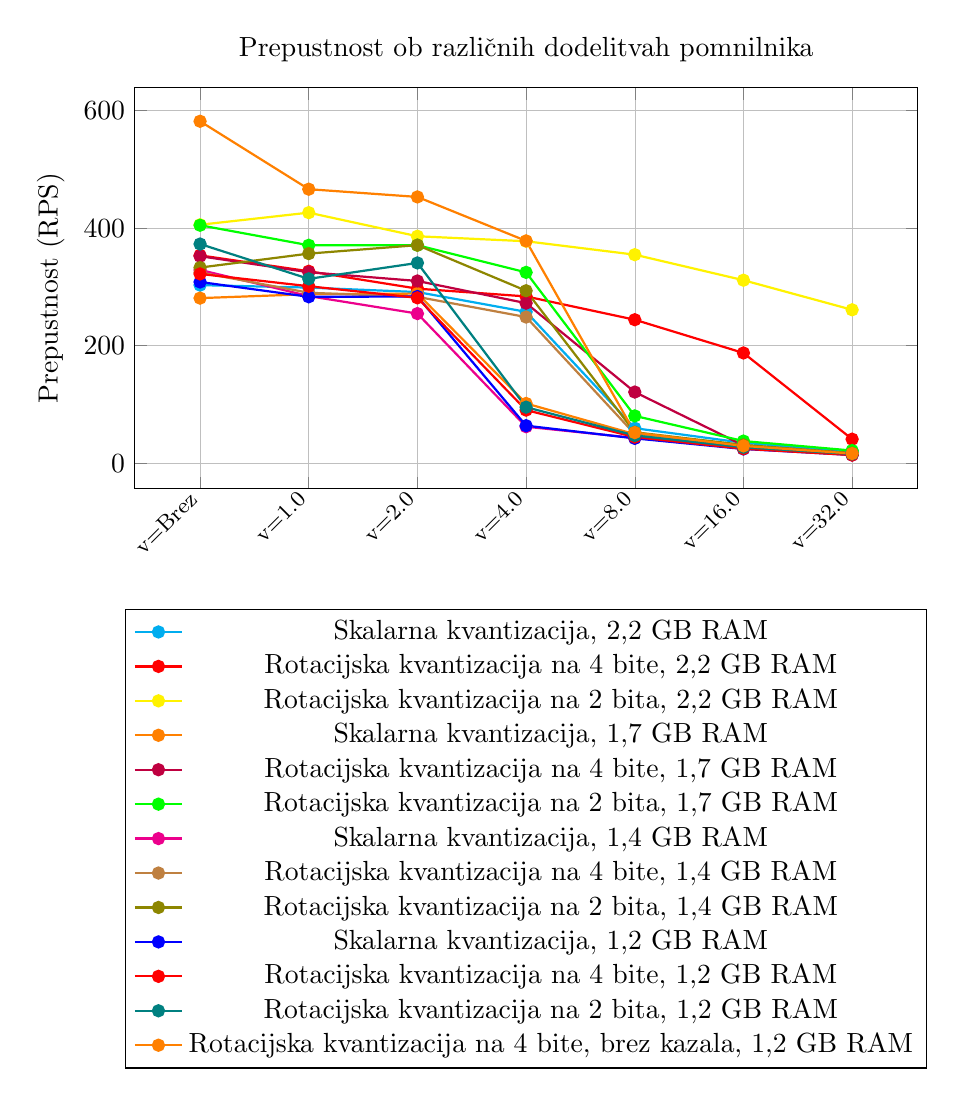
\begin{tikzpicture}
    \begin{axis}[
      title={Prepustnost ob različnih dodelitvah pomnilnika},
      ylabel={Prepustnost (RPS)},
      symbolic x coords={
        vnull,
        v1.0,
        v2.0,
        v4.0,
        v8.0,
        v16.0,
        v32.0,
      },
      xticklabels={
        {v=Brez},
        {v=1.0},
        {v=2.0},
        {v=4.0},
        {v=8.0},
        {v=16.0},
        {v=32.0}
      },
      xtick=data,
      x tick label style={rotate=45, anchor=east, align=center, font=\footnotesize},
      /pgf/number format/use comma,
      /pgf/number format/fixed,
      /pgf/number format/precision=3,      grid=both,
      grid style={line width=.1pt, draw=gray!20},
      major grid style={line width=.2pt, draw=gray!50},
      legend style={at={(0.5, -0.30)}, anchor=north},
      width=0.95\textwidth,
      height=0.55\textwidth,
    ]

    % Series: Skalarna kvantizacija, 2, GB RAM
    \addplot[color=cyan, mark=*, thick] coordinates {
      (vnull, 303.1286)
      (v1.0, 298.9116)
      (v2.0, 291.3495)
      (v4.0, 257.6954)
      (v8.0, 59.8532)
      (v16.0, 35.0105)
      (v32.0, 20.6449)
    };
    \addlegendentry{Skalarna kvantizacija, 2,2 GB RAM}

    % Series: Rotacijska kvantizacija na 4 bite, 2,2 GB RAM
    \addplot[color=red, mark=*, thick] coordinates {
      (vnull, 353.7137)
      (v1.0, 326.6954)
      (v2.0, 297.1088)
      (v4.0, 283.9080)
      (v8.0, 244.2856)
      (v16.0, 187.7566)
      (v32.0, 41.1977)
    };
    \addlegendentry{Rotacijska kvantizacija na 4 bite, 2,2 GB RAM}

    % Series: Rotacijska kvantizacija na 2 bita, 2,2 GB RAM
    \addplot[color=yellow, mark=*, thick] coordinates {
      (vnull, 405.7338)
      (v1.0, 426.3216)
      (v2.0, 386.1879)
      (v4.0, 377.7223)
      (v8.0, 354.8914)
      (v16.0, 311.4694)
      (v32.0, 261.1585)
    };
    \addlegendentry{Rotacijska kvantizacija na 2 bita, 2,2 GB RAM}

    % Series: Skalarna kvantizacija, 1,7 GB RAM
    \addplot[color=orange, mark=*, thick] coordinates {
      (vnull, 281.0156)
      (v1.0, 287.7506)
      (v2.0, 288.7166)
      (v4.0, 101.9174)
      (v8.0, 49.6295)
      (v16.0, 29.3668)
      (v32.0, 16.9126)
    };
    \addlegendentry{Skalarna kvantizacija, 1,7 GB RAM}

    % Series: Rotacijska kvantizacija na 4 bite, 1,7 GB RAM
    \addplot[color=purple, mark=*, thick] coordinates {
      (vnull, 352.2756)
      (v1.0, 325.0040)
      (v2.0, 310.1677)
      (v4.0, 272.4349)
      (v8.0, 121.3210)
      (v16.0, 30.5835)
      (v32.0, 17.3329)
    };
    \addlegendentry{Rotacijska kvantizacija na 4 bite, 1,7 GB RAM}

    % Series: Rotacijska kvantizacija na 2 bita, 1,7 GB RAM
    \addplot[color=green, mark=*, thick] coordinates {
      (vnull, 404.9143)
      (v1.0, 370.8909)
      (v2.0, 370.9902)
      (v4.0, 324.7901)
      (v8.0, 80.7713)
      (v16.0, 37.9946)
      (v32.0, 21.8426)
    };
    \addlegendentry{Rotacijska kvantizacija na 2 bita, 1,7 GB RAM}

    % Series: Skalarna kvantizacija, 1,4 GB RAM
    \addplot[color=magenta, mark=*, thick] coordinates {
      (vnull, 328.9937)
      (v1.0, 284.4947)
      (v2.0, 254.7136)
      (v4.0, 62.3949)
      (v8.0, 43.2334)
      (v16.0, 25.8227)
      (v32.0, 15.0849)
    };
    \addlegendentry{Skalarna kvantizacija, 1,4 GB RAM}

    % Series: Rotacijska kvantizacija na 4 bite, 1,4 GB RAM
    \addplot[color=brown, mark=*, thick] coordinates {
      (vnull, 324.6550)
      (v1.0, 290.1410)
      (v2.0, 283.1567)
      (v4.0, 248.8283)
      (v8.0, 49.7628)
      (v16.0, 27.2354)
      (v32.0, 16.5459)
    };
    \addlegendentry{Rotacijska kvantizacija na 4 bite, 1,4 GB RAM}

    % Series: Rotacijska kvantizacija na 2 bita, 1,4 GB RAM
    \addplot[color=olive, mark=*, thick] coordinates {
      (vnull, 332.9773)
      (v1.0, 356.7020)
      (v2.0, 371.0703)
      (v4.0, 293.5404)
      (v8.0, 52.9437)
      (v16.0, 31.4480)
      (v32.0, 17.4162)
    };
    \addlegendentry{Rotacijska kvantizacija na 2 bita, 1,4 GB RAM}

    % Series: Skalarna kvantizacija, 1,2 GB RAM
    \addplot[color=blue, mark=*, thick] coordinates {
      (vnull, 308.4515)
      (v1.0, 283.2663)
      (v2.0, 283.7407)
      (v4.0, 64.1327)
      (v8.0, 42.5738)
      (v16.0, 24.5048)
      (v32.0, 14.3456)
    };
    \addlegendentry{Skalarna kvantizacija, 1,2 GB RAM}

    % Series: Rotacijska kvantizacija na 4 bite, 1,2 GB RAM
    \addplot[color=red, mark=*, thick] coordinates {
      (vnull, 322.1524)
      (v1.0, 301.2405)
      (v2.0, 281.5185)
      (v4.0, 90.6148)
      (v8.0, 44.7847)
      (v16.0, 24.9387)
      (v32.0, 14.1302)
    };
    \addlegendentry{Rotacijska kvantizacija na 4 bite, 1,2 GB RAM}

    % Series: Rotacijska kvantizacija na 2 bita, 1,2 GB RAM
    \addplot[color=teal, mark=*, thick] coordinates {
      (vnull, 372.9866)
      (v1.0, 313.7923)
      (v2.0, 340.8405)
      (v4.0, 95.5884)
      (v8.0, 47.4377)
      (v16.0, 27.4389)
      (v32.0, 16.0379)
    };
    \addlegendentry{Rotacijska kvantizacija na 2 bita, 1,2 GB RAM}

    % Series: Rotacijska kvantizacija na 4 bite, brez kazala, 1,2 GB RAM
    \addplot[color=orange, mark=*, thick] coordinates {
      (vnull, 581.7274)
      (v1.0, 466.2381)
      (v2.0, 453.0560)
      (v4.0, 378.2856)
      (v8.0, 52.2828)
      (v16.0, 29.6967)
      (v32.0, 16.7648)
    };
    \addlegendentry{Rotacijska kvantizacija na 4 bite, brez kazala, 1,2 GB RAM}
    \end{axis}
  \end{tikzpicture}
  \caption{Primerjava rps across configurations.}
  \label{fig:benchmark_todo_rps}
\end{figure}